\section{Theory Solver For Difference Logic}
\label{sec:topic}



\subsection{Notation}
Throughout this chapter the following notation is used:
\begin{itemize}
    \item $ \phi $ is a \emph{conjunction} of difference logic constraints.
    It is being checked for satisfiability.
    \item $ x - y \prec c $ is a general form
    of a constraint in $ \phi $ where $ \prec \; \in \{ <, \leq \} $.
    \item $ \mathbb{D} $ is a domain over which
    the variables and constants in $ \phi $ are defined
    (\eg $ \mathbb{R} $).
\end{itemize}



\subsection{Constraint Graph}
Constraint graph
is a weighted directed graph which represents $ \phi $
and which is used by a difference logic constraints checker
(Figure~\ref{fig:lazy-and-incremental-approaches}) to test
if $ \phi $ is SAT.
In~\cite{cotton2004some} it is defined as follows:
\begin{definition}[Constraint Graph]
    \label{def:constraint-graph}
    Constraint graph is a graph $ \Gamma = (V,E,weight,op) $ where:
    \begin{itemize}
        \item $ V $ is a set of vertices. Each vertex $ x \in V $
        corresponds to one numeric variable occurring in $ x - y \prec c $.
        \item $ E $ is a set of directed edges. Each edge
        $ (x,y) \in E $ corresponds to $ x - y \prec c $.
        \item $ weight(x,y): E \mapsto \mathbb{D} $ is a weight function.
        It maps each edge $ (x,y) \in E $ to the constant
        $ c \in \mathbb{D} $ from the corresponding DL inequality
        $ x - y \prec c $.
        \item $ op(x,y): E \mapsto \{ <, \leq \} $ is a function which
        maps each edge $ (x,y) \in E $ to the operation
        $ \prec $ from the corresponding DL inequality
        $ x - y \prec c $.
    \end{itemize}
\end{definition}

Examples of constraint graphs
are shown on Figure~\ref{fig:contraints-graphs}.
\begin{figure}[htb]
    \begin{center}
        \begin{tabular}{cc}
            \begin{minipage}{0.45\linewidth}
                \begin{center}
                    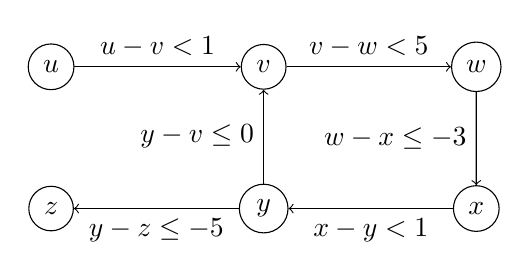
\begin{tikzpicture}[scale=0.9,state/.style={draw, circle, fill=none,text centered, text=black}]
    \node[state] (u) at (0, 2) {$u$};
    \node[state] (v) at (3, 2) {$v$};
    \node[state] (w) at (6, 2) {$w$};
    \node[state] (x) at (6, 0) {$x$};
    \node[state] (y) at (3, 0) {$y$};
    \node[state] (z) at (0, 0) {$z$};
    \draw [->] (u) -- node[anchor=south] {$ u-v < 1 $} (v);
    \draw [->] (v) -- node[anchor=south] {$ v-w < 5 $} (w);
    \draw [->] (w) -- node[anchor=east] {$ w-x \leq -3 $} (x);
    \draw [->] (x) -- node[anchor=north] {$ x-y < 1 $} (y);
    \draw [->] (y) -- node[anchor=north] {$ y-z \leq -5 $} (z);
    \draw [->] (y) -- node[anchor=east] {$ y-v \leq 0 $} (v);
\end{tikzpicture}

                \end{center}
            \end{minipage}
            &
            \begin{minipage}{0.45\linewidth}
                \begin{center}
                    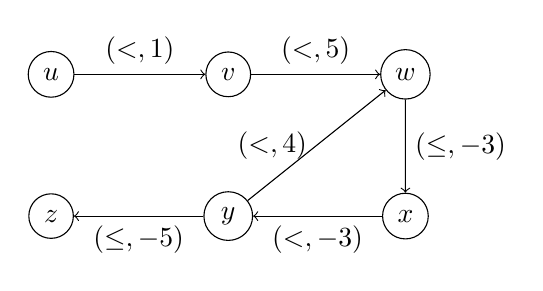
\begin{tikzpicture}[scale=0.9,state/.style={draw, circle, fill=none,text centered, text=black}]
    \node[state] (u) at (0, 2) {$u$};
    \node[state] (v) at (2.5, 2) {$v$};
    \node[state] (w) at (5, 2) {$w$};
    \node[state] (x) at (5, 0) {$x$};
    \node[state] (y) at (2.5, 0) {$y$};
    \node[state] (z) at (0, 0) {$z$};
    \draw [->] (u) -- node[anchor=south] {$ (<,1) $} (v);
    \draw [->] (v) -- node[anchor=south] {$ (<,5) $} (w);
    \draw [->] (w) -- node[anchor=west] {$ (\leq,-3) $} (x);
    \draw [->] (x) -- node[anchor=north] {$ (<,-3) $} (y);
    \draw [->] (y) -- node[anchor=north] {$ (\leq,-5) $} (z);
    \draw [->] (y) -- node[anchor=east] {$ (<,4) $} (w);
\end{tikzpicture}

                \end{center}
            \end{minipage}
        \end{tabular}
    \end{center}
    \caption{Examples of constraint graphs for
        Equation~\ref{eq:example-1} (left) and
        Equation~\ref{eq:example-2} (right).}
    \label{fig:contraints-graphs}
\end{figure}



\subsection{Negative Cycles in Constraint Graph}
A path in a constraint graph
can be used to infer a
new inequality by applying
transitivity rule
(Equation~\ref{eq:transitivity-example}).
The path
$ u \rightarrow v \rightarrow w \rightarrow x $
in the left graph on Figure~\ref{fig:contraints-graphs}
exemplifies it:

\begin{equation}
\begin{aligned}
u - v & < \;\;\; 1 \\
v - w & < \;\;\; 5 \\
w - x & \leq -3 \\
\hline
u - x & < \;\;\; 3
\end{aligned}
\end{equation}

If at least one strict inequality is present
then the resulting inequality will also be strict.

In~\cite{cotton2004some} it is shown
that a negative cycle
in a constraint graph
corresponds to a conflict
of the form $ 0 \prec c $
where $ c < 0 $.
Therefore if a constrain graph has a negative cycle
then the corresponding formula $ \phi $ is unsatisfiable.
In the same paper it is also shown
that if the graph has a zero weight cycle
then it corresponds to an inequality
$ 0 \prec 0 $ which represents a conflict
in case when $ \prec \; = \; < $ \ie when the
inequality is strict.
In this case $ \phi $ is also unsatisfiable.
This case also shows why one needs
to map edges of a constraint graph
not only into constants but also
into types of inequalities (strict or
non-strict, function $ op $
in the Definition~\ref{def:constraint-graph}).

An example of a conflict can be seen on the right graph
on Figure~\ref{fig:contraints-graphs}.
The conflict corresponds to the negative cycle
$ x \rightarrow y \rightarrow w \rightarrow x $
which corresponds to the following conflicting inequalities:

\begin{equation}
    \begin{aligned}
        x - y & < -3 \\
        y - w & < \;\;\; 4 \\
        w - x & \leq -3 \\
        \hline
        0 & < -2
    \end{aligned}
\end{equation}

The bottomline: $ \phi $ is unsatisfiable iff the
corresponding constraint graph has a negative
cycle or a zero weight cycle with at least
one strict inequality in it.



\subsection{Bellman-Ford Algorithm for Constraint Graph}
\cite{cotton2004some} uses a Goldberg-Radzik~\cite{goldberg1993heuristic}
variant of the Bellman-Ford algorithm~\cite[p.651]{cormen2009introduction}
to detect negative and zero weight cycles
and thus check if $ \phi $ is satisfiable
(Algorithm~\ref{alg:goldberg-radzik}).
\cite{goldberg1993heuristic}~states that the algorithm has the same
worst-case complexity $ O(|V| \cdot |E|) $
as Bellman-Ford algorithm but is superior in practice.
Terminology and notation used in the algorithm are given
in the definitions below:

\begin{Algorithm}
    \caption{An algorithm for checking if $ \phi $ which corresponds
        to the input constraint graph $ \Gamma = (V,E,weight,op) $ is satisfiable.
        It returns SAT or UNSAT status and a set of DL constraints
        corresponding to a conflict (in case of UNSAT).
        It is based on Bellman-Ford
        algorithm~\cite[p.561]{cormen2009introduction}.
        Goldberg-Radzik heuristic~\cite{goldberg1993heuristic},
        which is used here,
        suggests to scan a graph in a topological order.
        This algorithm uses
        depth first search~\cite[p.603]{cormen2009introduction} (DFS)
        and breadth first search~\cite[p.594]{cormen2009introduction} (BFS)
        for auxiliary tasks.
        $ \Gamma_d $ is the dynamically changing
        admissible graph
        from Definition~\ref{def:admissible-graph}.
    }
    \label{alg:goldberg-radzik}
    \begin{algorithm}{Goldberg-Radzik}
        {\text{constraint graph} \Gamma = (V,E,weight,op),
            \text{source vertex} s \in V}
        \begin{FOR}{\mathrm{each \; vertex} \; x \in V}
            d(x) = \infty \\
            status(x) = unreached
        \end{FOR} \\
        d(s) = 0 \\
        status(s) = labeled \\
        A \= \varnothing \\
        B \= \{ s \} \\
        \begin{REPEAT} \\
            \begin{IF}{\Gamma_d \text{has a cycle} C \text{(DFS on} \Gamma_d \text{can be used to check it)}}
                l \= \text{length of} C \text{in} \Gamma \\
                \begin{IF}{l < 0}
                    \RETURN (UNSAT, \text{DL constraints corresponding to} L)
                \end{IF} \\
                \begin{IF}{\exists \; (x,y) \in L \text{such that} op(x,y) = \; <}
                    \RETURN (UNSAT, \text{DL constraints corresponding to} L)
                \end{IF}
            \end{IF} \\
            \begin{FOR}{\mathrm{each \; vertex} \; x \in B}
                \begin{IF}{x \text{has no outgoing admissible edges}}
                    B \= B \setminus \{ x \} \\
                    status(x) = scanned
                \end{IF}
            \end{FOR} \\
            A \= \text{set of unexplored vertices reachable from}
            B \text{in} \Gamma_d
            \text{(BFS on} \Gamma_d \text{can be used here)} \\
            A \= \text{sort} A \text{topologically using}
            \Gamma_d \text{as an input graph}
            \text{(DFS on} \Gamma_d \text{can be used here)} \\
            B \= \varnothing \\
            \begin{FOR}{\mathrm{each \; vertex} \; x \in A}
                status(x) = labeled \\
                \begin{FOR}{\mathrm{each \; edge} \; (x,y) \in E}
                    \begin{IF}{d(x) + weight(x,y) < d(y)}
                        d(y) \= d(x) + weight(x,y) \\
                        \begin{IF}{status(y) = unreached}
                            B \= B \cup \{ y \}
                        \end{IF} \\
                        status(y) \= labeled \\
                        status(x) \= scanned
                    \end{IF}
                \end{FOR}
            \end{FOR}
        \end{REPEAT} A \; is \; empty \\
        \RETURN (SAT, \varnothing) \\
    \end{algorithm}
\end{Algorithm}

\begin{definition}[Source Vertex]
    The source vertex $ s \in V $ is a vertex from which
    the shortest paths to other vertices are computed.
\end{definition}

\begin{definition}[Distance Estimating Function~\cite{cotton2004some}]
    The distance estimating function $ d(v): V \mapsto \mathbb{D} $
    is a function which returns an upper bound
    on the length of the shortest path
    from the source vertex to the given vertex $ v \in V $.
\end{definition}

\begin{definition}[Reduced Cost Function~\cite{goldberg1993heuristic}]
    The reduced cost function
    $ r(x,y): V \mapsto \mathbb{D} $ is
    defined as follows:
    $ r(x,y) = weight(x,y) + d(x) - d(y) $.
\end{definition}

\begin{definition}[Admissible Edge]
    Edge $ (x,y) \in E $ is called admissible if $ r(x,y) \leq 0 $.
\end{definition}

\begin{definition}[Admissible Graph]
    \label{def:admissible-graph}
    Admissible graph $ \Gamma_d $ is a subgraph
    of $ \Gamma $ composed of the admissible edges of $ \Gamma $.
\end{definition}

\begin{definition}[Vertex Status]
    The vertex status
    $ status(x) = \{ unreached, labeled, scanned \} $
    is a function on vertices which shows a current state of
    a vertex $ x \in V $.
    $ status(x) = unreached $ means $ x $ has not been explored yet.
    $ status(x) = labeled $ means $ x $ has been explored \ie
    the distance estimate for it has been updated at least once
    and potentially it can be used to improve distance estimates to
    other vertices.
    $ status(x) = scanned $ means $ x $ has been completely explored
    and will not be considered further for improving distance estimates.
\end{definition}

Algorithm~\ref{alg:goldberg-radzik} relies on
the following theorem:

\begin{theorem}
    \label{the:neg-cycle-in-cg}
    Given a constraint graph $ \Gamma $ and a series of distance estimating
    functions $ (d_0, d_1, d_2, d_3, \dots) $, $ \Gamma $ has a negative
    or zero cycle if and only if $ \Gamma_d $ has a cycle under some
    distance estimate $ d_k $.
\end{theorem}

Theorem~\ref{the:neg-cycle-in-cg} is proven
in~\cite{cotton2004some}.
The intuition behind it is the following.
$ \Gamma_d $ consists of edges which may
potentially improve some current distance estimate
function $ d_k $.
If $ \Gamma_d $ has a cycle then it means that this
cycle may potentially be used to update
the distance estimate function $ d_k $
infinitely many times thus preventing the
process from convergence.
As stated in~\cite[p.645]{cormen2009introduction}
inability to converge means that the single-source
shortest paths problem is not well defined
which means that there has to be a negative weight
cycle which can always be used to improve
distance estimates.

The whole satisfiability checking process
of a difference logic formula
(Figure~\ref{fig:lazy-and-incremental-approaches},~right)
can be approximately described as follows:

\begin{itemize}
    \item A boolean skeleton $ \phi' $ is built.
    \item The SAT solver starts solving $ \phi' $.
    \item When it modifies a current variables assignment,
    it maps it to a conjunction of difference logic
    inequalities and tells the constraints checker
    what new inequalities need to be added
    and what previously passed inequalities
    need to be deleted.
    \item The constraints checker modifies its
    state accordingly (\ie the constraint graph
    and other data structures).
    \item The constraints checker tries to
    find a negative or zero cycle
    which would correspond to a conflict
    (Algorithm~\ref{alg:goldberg-radzik}).
    \begin{itemize}
        \item If it runs into such a conflict
        then it informs the SAT checker
        and returns it the inequalities
        which constitute the cycle
        as the explanation of
        the encountered conflict.
        \item Otherwise it informs the SAT checker
        that the current variables assignment
        is consistent with the theory
        (the $ \algCALL{Theory} $ call
        in Algorithm~\ref{alg:basic-sat})
        and the SAT checker continues to
        search for a solution.
    \end{itemize}
\end{itemize}

The described process ends in two cases.
Either a complete solution is found,
which is also consistent with the theory.
It means that the input difference logic formula
is satisfiable.
Or the SAT solver has run into a conflict
which is impossible to resolve.
It means that the initial formula contains
a contradiction and thus is unsatisfiable.

As an example consider the difference logic formula
in Equation~\ref{eq:example-2} as an input:
\begin{itemize}
    \item $ \phi' = p_{u,v,1} \land p_{v,w,5} \land p_{w,x,-3} \land p_{x,y,-3} \land p_{y,z,-5} \land p_{y,w,4} $
    \item The SAT solver starts with a partial assignment
    $ \{ p_{u,v,1} = True \} $.
    It tells the constraints checker:
    "add $ (u - v < 1) $ and check consistency".
    \item The constraints checker adds the edge $ (u,v) $
    to the (initially empty) constraints graph,
    which corresponds to the received inequality.
    There are no cycles in the graph and therefore
    the constraints checker informs the SAT checker
    that the current variables assignment is consistent
    with the theory.
    \item The SAT solver continues searching
    for a solution.
    It extends a partial assignment to the following
    assignment:
    $ \{ p_{u,v,1} = True, p_{v,w,5} = True \} $.
    It tells the constraints checker:
    "add $ (v - w < 5) $ and check consistency".
    \item ...
    \item At some moment the SAT solver arrives
    in a state when it has
    $ \{ p_{u,v,1} = True, p_{v,w,5} = True, p_{w,x,-3} = True, p_{x,y,-3} = True, p_{y,z,-5} = True \} $
    as the current variables assignment and
    it extends it with an assignment $ p_{y,w,4} = True $.
    It tells the constraints checker:
    "add $ (y - w < 4) $ and check consistency".
    \item The constraints checker adds
    the new edge $ (y,w) $ and finds a negative cycle
    $ w \rightarrow x \rightarrow y \rightarrow w $
    corresponding to a conflict.
    The set of inequalities $ \{ (w - x \leq -3),
    (x - y < -3),
    (y - w < 4) \} $ correspond to the detected conflict.
    The constraints checker returns the explanation
    to the SAT solver:
    $ \neg ( p_{w,x,-3}
    \land p_{x,y,-3}
    \land p_{y,w,4} ) $
    which can be rewritten as
    $ ( \neg p_{w,x,-3}
    \lor \neg p_{x,y,-3}
    \lor \neg p_{y,w,4} ) $.
    \item The SAT solver adds the received explanation to
    $ \phi' $:
    \begin{equation}
        \phi'' = \phi' \land ( \neg p_{w,x,-3}
        \lor \neg p_{x,y,-3}
        \lor \neg p_{y,w,4} )
    \end{equation}
    Then it backtracks to the decision level 0
    and starts solving $ \phi'' $.
    It calls $ \algCALL{Propagate} $
    from Algorithm~\ref{alg:basic-sat}
    and runs into a conflict.
    The conflict cannot be resolved because
    it is detected on the decision level 0.
    Therefore the SAT solver returns
    UNSAT as the answer \ie the input
    difference logic formula from
    Equation~\ref{eq:example-2}
    is unsatisfiable.
\end{itemize}